%=========================Preamble====================================%
\documentclass[12pt] {article}
\usepackage{times}
\usepackage[margin=1in,bottom=1in,top=0.5in]{geometry}

\usepackage{graphicx}


\usepackage{float}
\usepackage{graphicx}
\usepackage{subfig}
\usepackage{wrapfig,lipsum}
\usepackage{amssymb}
\usepackage{nath}
\usepackage{amsfonts}


%=========================Doc====================================%
\begin{document}
\title{ECE 289A - An Introduction to Reinforcement Learning HW\#4}

\author{Ahmed H. Mahmoud}
\date{November, 9th 2017} 
\maketitle
\section*{Q.1}
In this question, we regenerated plot in Figure 6.5 in the book. Figure \ref{fig:a} shows the regenerated plots. In order to run the code, please make sure to install MATLAB \emph{Curve Fitting Toolbox} package which is used to smooth the curves. 

\begin{figure}[!tbh]
\centering        
   \subfloat {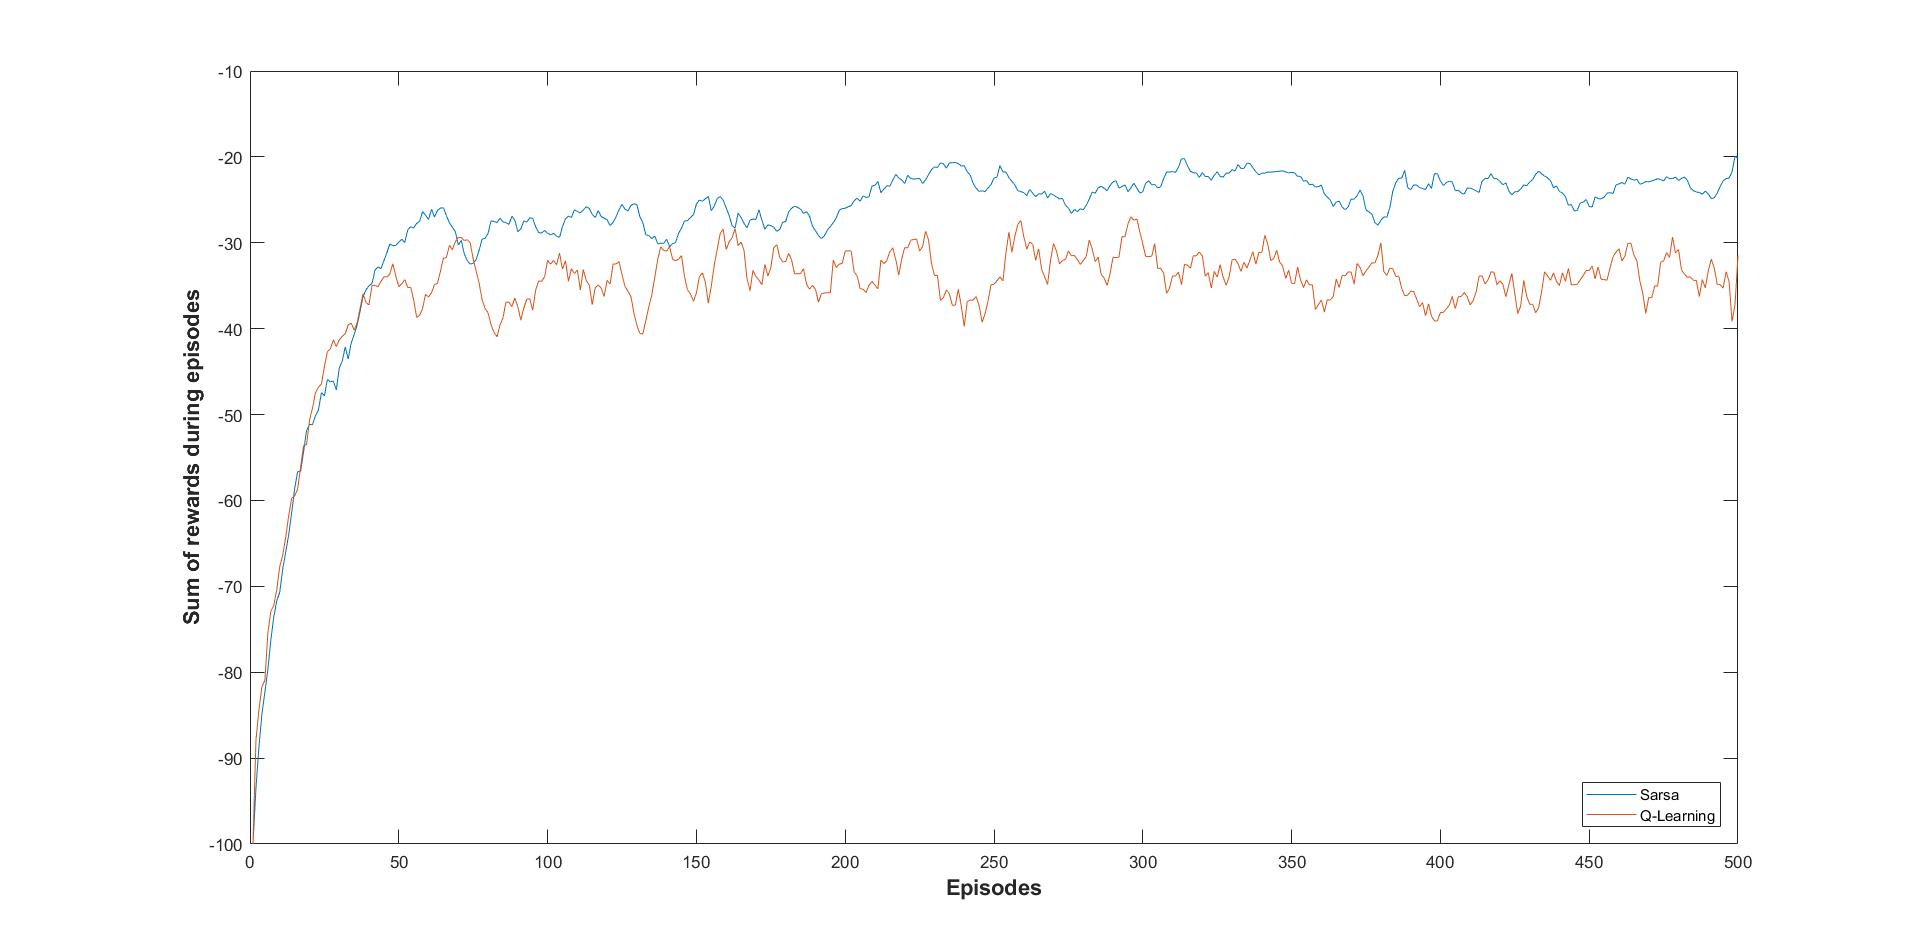
\includegraphics[width=0.9\textwidth]{../fig6_5.jpg}}  
   \caption{}
   \label{fig:a}
\end{figure}

\section*{Q.2}
Figure \ref{fig:b} shows the regenerate plot from Figure 7.2 in the book. 

\begin{figure}[!tbh]
\centering        
   \subfloat {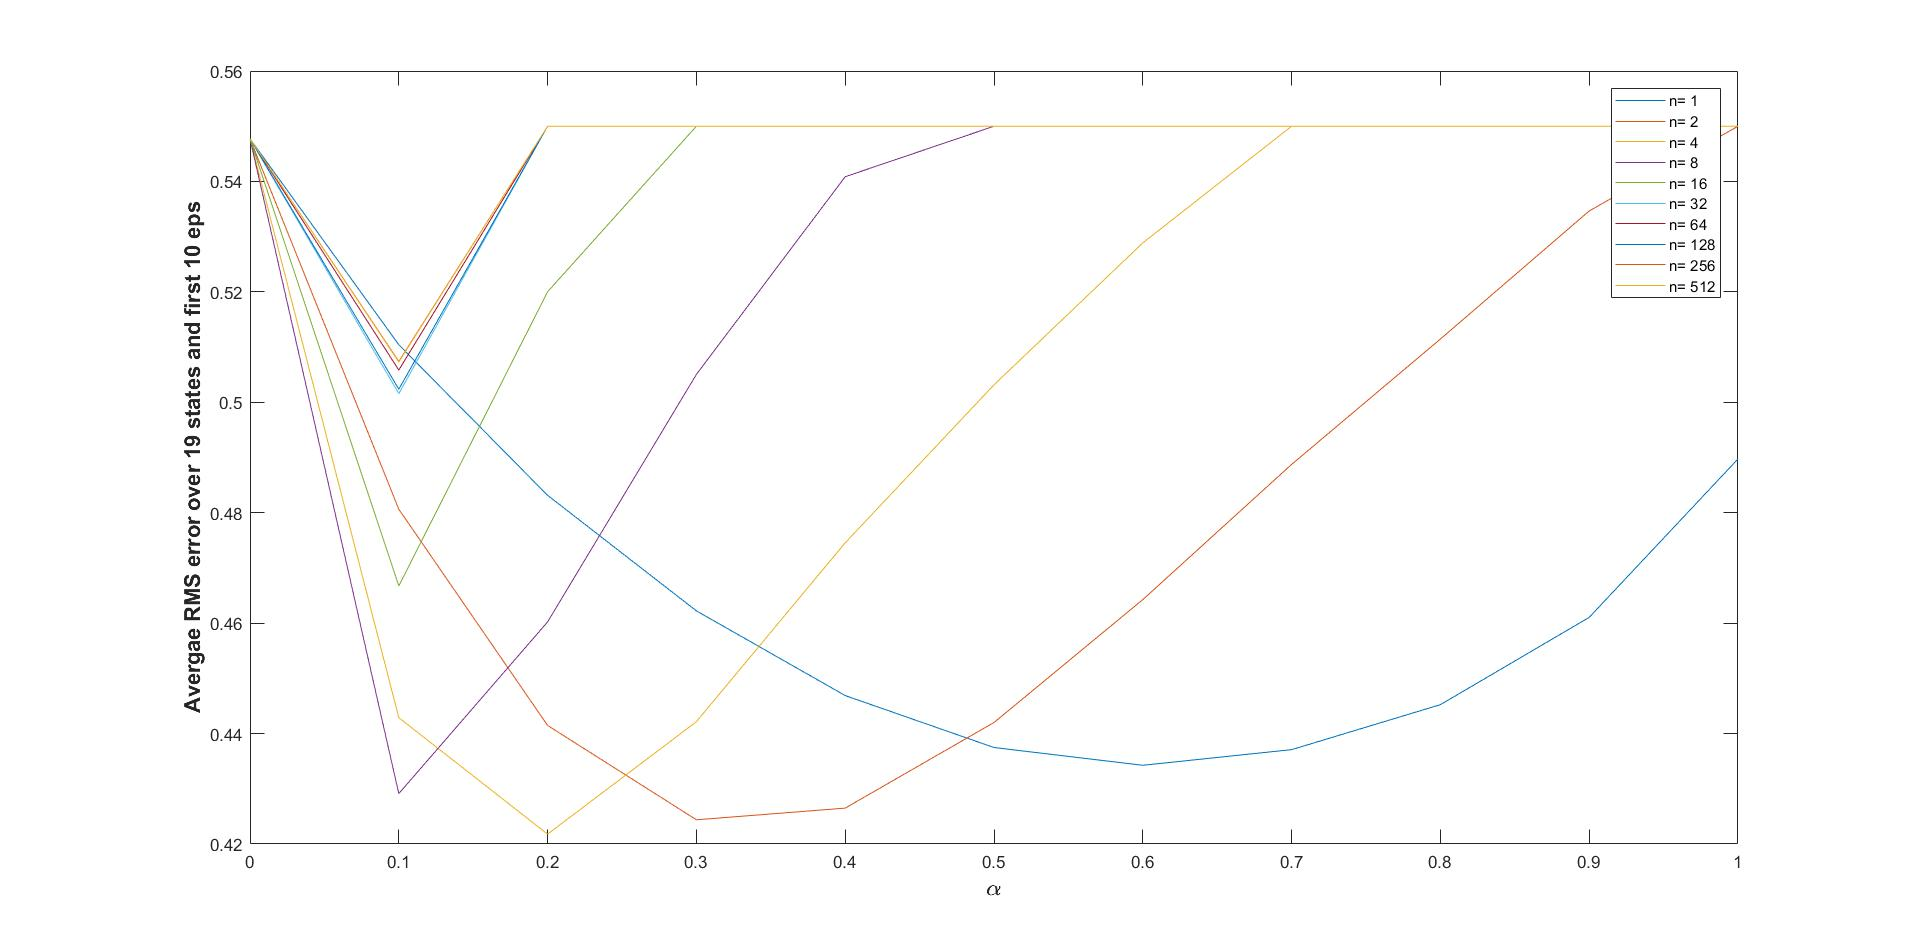
\includegraphics[width=0.9\textwidth]{../fig7_2.jpg}}        
   \caption{Performance of n-step TD methods as a function of $\alpha$ for various values of n on a 19-state random walk task.}
   \label{fig:b}
\end{figure}

\section*{Q.3}
Proving the following inequality for 

\[
max_{s}|\mathbb{E}_{\pi} \left[ G_{t:t+n}|S_{t}=s \right] - v_{\pi}(s)| \leq \gamma^{n}max_{s}|V_{t+n-1}(s)-v_{\pi}(s)|
\]
We start by expanding the error estimation 

\[
max_{s}|\mathbb{E}_{\pi} \left[ R_{t+1} + \gamma R_{t+2}+ \cdots + \gamma^{n-1} R_{t+n} + \gamma^{n}V_{t+n-1}(S_{t+n})| S_{t}= s \right]  - v_{\pi}(s)|
\]

In the limit, this quantity should always be less than $\gamma^{n}max_{s}|V_{t+n-1}(s)-v_{\pi}(s)|$ since for any stat $s$, the accumulated discounted rewards will provide a correction for the estimated $v_{\pi}(s)$.

\end{document}
